%! Author = joels
%! Date = 27/01/2022

\section{Objekt Orientierung}
\begin{minipage}{0.4\linewidth}
    \textbf{OO in Lexer \& Parser}
    \begin{itemize}[topsep=0pt]
        \itemsep -0.2em
        \item new-Operator für Klassen (new Point())
        \item Indirekte Zugriffsausdrücke (Designators)
        \item Type Cast und instanceof-Operator
    \end{itemize}
\end{minipage}
\begin{minipage}{0.6\linewidth}
    \textbf{OO in Semantic Checker}
    \begin{itemize}[topsep=0pt]
        \itemsep -0.2em
        \item Zuweisungs-Kompatibilität der Typen
        \SubItem{null passt auf alle Referenztypen}
        \SubItem{Subklasse passt auf Basisklasse (impl. Upcast)}
        \item Zuweisungen/Parameterübergabe/Rückgabe
        \item Vergleiche zwischen 2 Variablen: Gegenseitig zuweisungskompatibel
        \item Keine zyklische Vererbung
        \item Overriding stimmt: Gleiche Signatur/Return value
    \end{itemize}
\end{minipage}

\subsection{Heap}
\textbf{Ablage erzeugter Objekte auf dem Heap.} $\rightarrow$ Linearer Adressraum\\
\textbf{Warum nicht auf Stack?} Würden sonst verloren gehen wenn das Activation Frame abgebaut wird. $\rightarrow$ Nicht mehr an Methodeninkarnation gebunden\\
\textbf{Objekt-referenzen:}
\begin{itemize}[topsep=0pt]
    \itemsep -0.2em
    \item Verweis zum Objekt im Heap
    \SubItem{Repräsentiert durch Speicheradresse des Objektes}
    \item Variablen speichern nur Referenzen
    \SubItem{Falls vom referenztyp, d.h. Klasse, Array, String}
\end{itemize}
\subsubsection{Raw Heap}
\begin{itemize}[topsep=0pt]
    \itemsep -0.2em
    \item 64-Bit Adressen/Pointer
    \item Raw Heap kann keine Java referenzen speichern
    \SubItem{Sonst würde der GC im Managed Bereich nicht mehr funktionieren}
    \item Stattdessen Map (z.B. HashMap<Long, Object>) verwenden
\end{itemize}
\begin{minipage}{0.5\linewidth}
    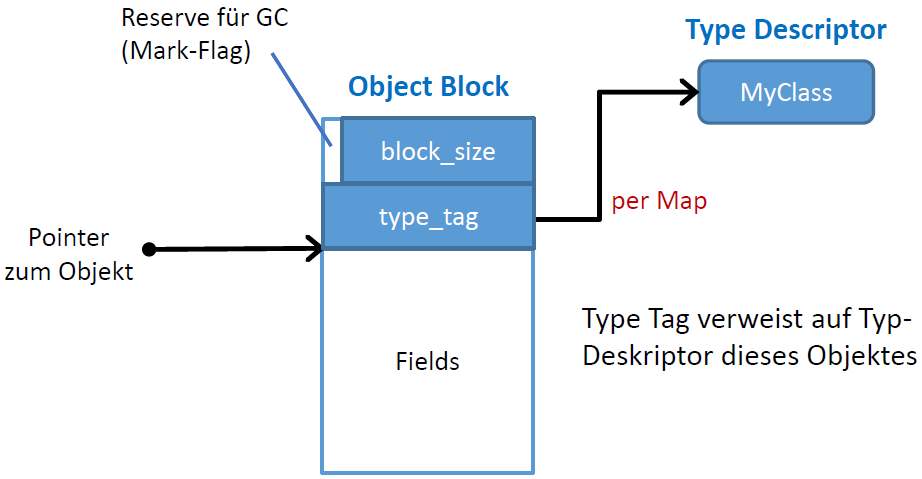
\includegraphics[width=\linewidth]{raw_heap}
\end{minipage}
\begin{minipage}{0.5\linewidth}
    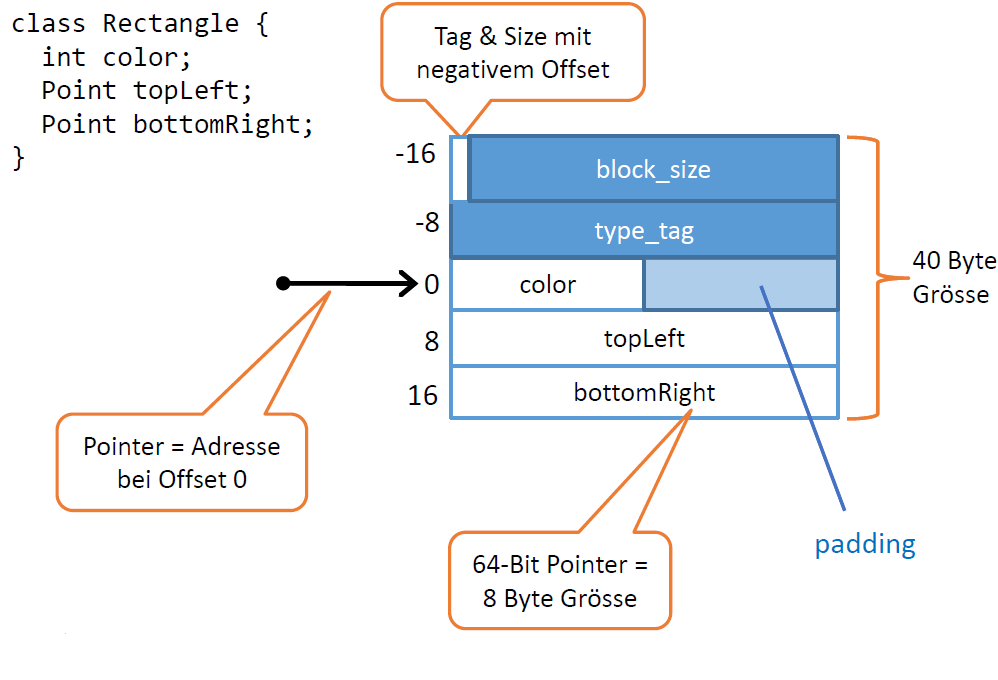
\includegraphics[width=\linewidth]{raw_heap_2}
\end{minipage}

\subsubsection{Einfache Heap Allokation}
\begin{lstlisting}
Pointer allocate(int size, TypeDescriptor type) {
    int blockSize = size + 16 // Mit Header
    if (freePointer + blockSize > limit) {
        throw new VMException("Out of Memory"); // Ohne GC
    }
    long address = freePointer;
    freePointer += blockSize;
    heap.setLong(address, blockSize);
    setTypeDescriptor(type, address); // at offset 8
    address += 16;
    return new Pointer(address);
}
\end{lstlisting}